\newpage
\chapter{Desenvolvimento}
\label{ch:desenvolvimento}

\par Este capítulo apresenta as etapas do desenvolvimento da biblioteca ICan.js

\section{Arquitetura da biblioteca}

% Não seguiu-se nenhum modelo proposto, apenas incorporou a estrutura descrita no artigo...
\par Para iniciar o desenvolvimento da biblioteca, fez-se inicialmente a definição de sua arquitetura. Nesta a biblioteca foi dividida em camadas, seguindo o modelo proposto por \citeonline{tensorflowjs2019}. Para este caso as camadas são a \textitbf{Core} e \textitbf{Common}, apresentadas na Figura \ref{figure:icanjsarch}.

\image{0.3}{tfjs-core.png}{Arquitetura do ICan.js}{figure:icanjsarch}{Adaptado de Google.com}

\par A camada \textitbf{Core} disponibiliza funcionalidades base, como os modelos de rede neural e regressão, assim como funcionalidades de calibração da regressão e de acesso a \textit{webcam} do usuário. Já a camada \textitbf{Common} utiliza os recursos do \textitbf{Core} para a criação dos recursos assistivos e disponibilização dos mesmos de forma facilitada.

\par Para a exposição de cada um dos componentes presentes em cada camada, as seções seguintes apresentam os recursos assistivos bem como as etapas de seu desenvolvimento e aplicação na biblioteca.

\section{Tradução de Libras para Texto}

% Devo colocar aqui algum texto descrevendo o recurso assistivo ? (10/03/2019)
\par Este recurso assistivo permite a interação dos usuários com deficiência auditiva a páginas da \textit{web} através de gestos de Libras. 

\subsection{Aquisição dos dados}

\par O grande desafio para o desenvolvimento deste recurso assistivo foi a base de dados, já que, o que tange o conhecimento do autor, não há bases de dados de gestos de Libras publicamente disponível, de modo a ser necessário a criação de uma base de dados para este trabalho.

% Redes neurais de classificação continua ?
\par Para este trabalho utilizou-se gestos que podem ser reconhecidos com apenas um \textit{frame}, sendo eles (a) Amigo, (b) Desculpa, (c) Telefone \cite{Magalh2018}. A Figura \ref{figure:gestos_selecionados} apresenta cada um dos gestos.

\begin{figure}[H]%
    \centering
    \subfloat[Amigo]{{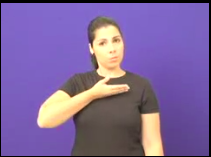
\includegraphics[height=3cm, width=5cm]{src/images/amigo.png}}}%
    \qquad
    \subfloat[Desculpa]{{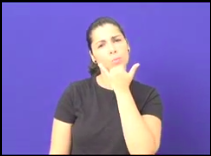
\includegraphics[height=3cm, width=5cm]{src/images/desculpa.png} }}%
    \qquad
    \subfloat[Telefone]{{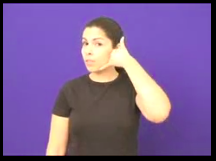
\includegraphics[height=3cm, width=5cm]{src/images/telefone.png} }}%
    \qquad
    \caption{Gestos selecionado para o conjunto de dados}%
    \label{figure:gestos_selecionados}%
    \fonte{Produção do autor} % Adaptado de Dicionário de Libras
\end{figure}

\par Para a aquisição dos dados, foi desenvolvido uma ferramenta (Figura \ref{figure:sistema_aquisicao}) \textit{desktop} multiplataforma na linguagem Python, com o auxílio da biblioteca PyQt, para a criação da interface gráfica e a biblioteca OpenCV, para a manipulação das imagens capturadas.

% Ei!! Problema na imagem, você não declarou ter utilizado o gesto "Idade".... (07/03/2019)
\image{0.60}{image_sistema_aquisicao_de_dados.png}{Tela inicial da aplicação de aquisição de dados}{figure:sistema_aquisicao}{Produção do Autor}

\par Como apresentado na Figura \ref{figure:sistema_aquisicao}, o sistema de aquisição de imagens demonstra exemplos dos gestos que devem ser reproduzidos pelo usuário, uma barra de progresso, e botões para recomeçar a captura ou saber mais sobre o projeto, além da imagem do próprio usuário.

\par Este sistema captura 60 imagens, sendo 20 de cada um dos gestos, em cada uma das imagens capturadas é aplicado uma operação de redimensionamento, isto para que, todas as imagens tenham as dimensões 224x224x3, já que esta é a dimensão aceita pelo \textit{Mobilenet}, o mesmo que será retreinado com os dados que estão sendo coletados. Após a aquisição das 60 imagens o programa cria um arquivo no formato zip e o envia para um \textit{email} criado para o armazenamento dos dados.

\par O programa foi distribuído e ao final houveram 11 colabores, criando assim um conjunto com 660 imagens.

\subsection{Pré-processamento dos dados} 

\par Durante a aquisição das imagens, nenhuma restrição foi emposta aos colaboradores, assim uma etapa de validação de cada uma das imagens teve de ser realizada para garantir que, cada uma das imagens representa o gesto ao qual é indicado, o que resultou na remoção de algumas imagens. A Figura \ref{figure:plot_qtd_apos_filtro} apresenta a relação da quantidade de imagens com cada um dos gestos após a validação realizada.

% Imagem aqui
\image{0.30}{tem_grafico_de_barra.PNG}{Quantidade de imagens por gesto após filtragem}{figure:plot_qtd_apos_filtro}{Produção do Autor}

% Como posso escrever que, isto está sendo feito já que após testes houveram problemas?? Posso escrever aqui mesmo ? ? ?
\par A quantidade de imagens disponíveis após o filtro pode representar problemas para a generalização do modelo, mesmo levando em consideração o retreino que será feito, desta forma será aplicado a técnica de \textit{Data Augmentation}, esta que aumenta a quantidade de imagens realizando modificações com filtros e alterações na base já existente.

\par Neste trabalho, o \textit{Data Augmentation} foi realizado com o auxílio do \textit{Augmentor}, uma biblioteca Python que permite a criação de um \textit{Pipeline} de alterações baseado em probabilidade, assim atribui-se para cada alteração que pode ser aplicada na imagem uma probabilidade de ocorrência, e então o \textit{Augmentor} através destas aplica uma ou várias alterações na base de imagens. A Figura \ref{figure:dataaugmentation} apresenta o código aplicado para esta atividade.

\begin{figure}[H]
    \centering
    \begin{lstlisting}[language=Python]
import Augmentor

p = Augmentor.Pipeline('gestos_editados/treino')

p.flip_left_right(probability=0.6)

p.rotate(probability=0.7, max_left_rotation=3, max_right_rotation=3)
p.rotate(probability=0.4, max_left_rotation=7, max_right_rotation=7)

p.random_distortion(probability=0.5, grid_height=3, grid_width=3, magnitude=2)
p.random_distortion(probability=0.4, grid_height=4, grid_width=4, magnitude=3)

p.skew_left_right(probability=0.3, magnitude=0.7)
p.skew_corner(probability=0.4, magnitude=0.5)

p.shear(probability=0.5, max_shear_left=4, max_shear_right=3)

p.sample(1500)
    \end{lstlisting}
    \caption{\textit{Script} de \textit{Data Augmentation}}
    \label{figure:dataaugmentation}
\end{figure}

\par Veja que, cria-se inicialmente uma instância de \textit{Pipeline} indicando apenas o diretório das imagens de treino, e então todas as possíveis modificações são declaradas na instância de \textit{Pipeline} e junto a cada uma delas uma probabilidade. No fim, é indicado que o total de imagens gerado deve ser 1500.

% Após finalizar esta versão iterar colocando uma tabela com cada operação aplicada no Pipeline, com imagens de exemplo inclusive.. (09/03/2019).

\par Após a aplicação do \textit{Pipeline} o conjunto de treinamento passou a ter 1500 imagens, a Figura \ref{figure:plot_qtd_apos_dataaugmentation} mostra este valor distribuído por gesto.

% Imagem aqui
\image{0.30}{tem_grafico_de_barra.PNG}{Quantidade de imagens por gesto com \textit{Data Aumentation}}{figure:plot_qtd_apos_dataaugmentation}{Produção do Autor}

\subsection{Treinamento da Rede Neural Convolucional}

% Falar sobre o treinamento

\subsection{Distribuição do modelo}

% Posso falar da transformação aqui também...
% Com a finalização do treinamento, o modelo foi salvo inicialmente no formato \textit{h5}, porém para que o mesmo possa ser utilizado fez-se a transformação deste formato para um formato otimizado pela web...(Pegar nome algo assim....).
% Texto explicando para a avó
\par Para tornar a distribuição e utilização da biblioteca simples, foi criado uma \textit{API Rest} para a distribuição do modelo treinado, fazendo com que, os usuários da API não tenham que prover serviços de distribuição dos modelos.....
\par A \textit{API} foi criada utilizando \textit{Flask}, um \textit{microframework} Python para a realização de desenvolvimento web.

% Colocar imagem da página inicial da API... ou mesmo da página de exemplo e tals... Dar valor ao trabalho realizado.

\par O consumo desta \textit{API} é feito através do módulo \textitbf{MobileNetV1Libras} presente na camada \textitbf{Core} do ICan.js.

% Colocar código consumindo o modelo via API aqui....

\subsection{Criação do recurso assistivo}

% Explicando para a avó
\par Após todo o processo de treinamento do modelo de CNN utilizado neste recurso assistivo, foi adicionado na camada \textitbf{Common} da biblioteca o componente \textitbf{Writer}, este que permite a escrita em campos de uma página \textit{web} utilizando gestos de Libras.

% Falar do espaço de tempo....
\par O treinamento da CNN aplicada neste recurso assistivo, como demonstrado, utiliza imagens estáticas, porém para garantir a usabilidade, o método descrito por \citeonline{Magalh2018} é aplicado, desta forma, um conjunto de \textit{frames} é reconhecido pela rede neural e então a média dos resultados é utilizada para a escolha da palavra.

% \par Mesmo o treinamento da CNN aplicado neste recurso assistivo ter sido realizado com imagens estática, o módulo implementado recebe um \textit{stream} de vídeo. Isto porque o usuário define além do \textit{stream} a quantidade de \textit{frames} que deve ser levada em consideração e o tempo entre a aquisição de uma \textit{frame} e outro, fazendo assim com que, a média da classificação destes \textit{frames} seja utilizada como a palavra sendo representada no gesto, assim como apresentado em \cite{Magalh2018}.

\par Toda esta operação da captura de um conjunto de \textit{frames} é feito através de uma função recursiva, demonstrada na Figura \ref{figure:class_recursiva}.

% \par Toda esta operação da captura de \textit{frames} em um intervalo de tempo é feito através de uma função recursiva, demonstrada na Figura \ref{figure:class_recursiva}.

\begin{figure}[H]
    \centering
    \begin{lstlisting}[language=JavaScript]
async function recursiveInterval() {
    try {
        gestures.push(await mobilenetGestures.predictFrame());

        if (gestures.length >= nFrames) {
            // Tira a média de valores classificados
            fnc(getMeanGesture(gestures));
            gestures = [];
        }

        timeout = window.setTimeout(() => {
            recursiveInterval();
        }, delay * 1000);       
    } catch(err) {
        if (timeout !== null) {
            window.clearTimeout(timeout);
        }

        console.error("librasWriter", err);
    }
}
    \end{lstlisting}
    \caption{\textit{Script} de classificação recursiva}
    \label{figure:class_recursiva}
\end{figure}

% Explicação para a avó
% Na explicação final, não deixe de colocar explicações levando em consideração o código (Trechos e números de linhas).....
\par Veja que, a cada vez chamada a função recursiva, é feita uma classificação, e seu resultado é inserido em uma lista, após isto a quantidade de elementos dentro da lista é verificado, caso seja igual ou maior ao limite definido pelo usuário, é feito a média das classificações e então o resultado é devolvido ao usuário, caso contrário a função fica parada por um intervalo de tempo, definido pelo usuário e então após o intervalo a função é chamada novamente, repetindo todo o ciclo.

\section{Controle de \textit{mouse} com movimentos da cabeça}

\par Este recurso assistivo permite a interação de usuários com deficiência motora a navegação de páginas da \textit{web} com movimentos da cabeça.

\par O desenvolvimento deste recurso assistivo ocorreu através da utilização do modelo PoseNet junto a regressão linear.

% % Explicação para a avó
% \par Para isto o modelo identifica os pontos do corpo do usuário, os valores da posição do ponto identificado é aplicado em uma regressão, esta que devolve a posição a qual o usuário está  

\subsection{Mapeamento dos movimentos}

% Ao descrever melhor o mapeamento, dar mais enfâse para certas partes do código... Como a de classificação do PoseNet, já que houve um trabalho para a criação deste código....

% Explicação para a avó
\par O mapeamento dos movimentos do usuário para movimentos do mouse é feito através da integração do PoseNet e de regressão linear, como já explicado anteriormente.

\par Para este desenvolvimento, utilizou-se os conceitos apresentados por \cite{Papoutsaki2016}, onde o mapeamento dos gestos era feito utilizando diferentes modelos de regressão, porém neste trabalho utilizou-se apenas a regressão linear, e o método de identificação dos pontos do usuário, neste caso foi o PoseNet.

\par Com isto, há um módulo dentro do \textitbf{Core} da biblioteca nomeado PoseNet, que possui os mecanismos de utilização do PoseNet já implementado no TFJS. 

\par Desta forma, a saída da identificação do PoseNet, ou seja, a posição onde está a parte do corpo interessada, neste caso o nariz, passa como entrada para a regressão, que foi previamente calibrada para mapear a posição do mouse com a posição do nariz do usuário, desta forma é feita a predição da posição onde o usuário pode estar apontando o nariz.

\par Para as representações de regressão, dentro do \textitbf{Core} há o módulo \textitbf{Regression}, que possui as regressões.

% Mostrar código....

\subsection{Calibração da regressão}

\par Foi especificado que, utiliza-se de regressões para o mapeamento após a identificação feita com o PoseNet, porém estes modelos precisam de alguma forma serem calibrados e assim se ajustar as possibilidades de movimentação de cada usuário, para facilitar este processo de calibração o ICan.js fornece uma \textit{API} de calibração, esta presente na camada \textitbf{Core}.

% Colocar imagens...

% Imagem mostrando como funciona todo o processo...

% Veja que na figura acima

% Um dos grandes desafios do desenvolvimento dos recursos assistivos para deficientes auditivos foi a base de dados, isto porque o que tange o conhecimento do autor, não há nenhuma base de dados de imagens de sinais da Língua Brasileira de Sinais disponível publicamente, de modo a ser necessário a criação de uma base de dados própria.

% \par A especificação e desenvolvimento de cada uma das camadas será feita nas seções a frente.



% \subsection{Camada Core}

% A camada \textitbf{Core} da biblioteca ICan.js é responsável pelas principais funcionalidades

% \par Como apresentado na Figura \ref{figure:icanjsarch}, a camada \textitbf{Core} disponibiliza funcionalidades essenciais para a criação de recursos assistivos, com por exemplo, os modelos de rede neural e regressão, assim como facilidades para acesso e manipulação da \textit{webcam} do usuário. Por outro lado, a camada \textitbf{Common} apresenta funcionalidades de alto nível criadas utilizando o \textitbf{Core}, como por exemplo as funcionalidades de controle de \textit{mouse} através de movimentos com a cabeça, e transcrição de gestos de Libras para texto.

% \par As subseções a frente apresentam 


% % (23/02/2019) -> Talvez aplicar O NVIDIA Digits para demonstrar algumas coisas da rede, formas de identificação....Alguma coisa assim.... 

% % Colocar algum texto desta forma como está abaixo, ou algo assim....
% % Este capítulo apresenta os recursos assistivos que foram desenvolvidos durante a criação deste trabalho, como forma de confirmação dos estudos de casos levantados 
% % Este capítulo apresenta os processos de coleta e pré-processamento dos dados, treinamento e validação da CNN e o desenvolvimento da biblioteca ICan.js.

% % Conversando com Giuliano hoje (07/03/2019), ele me recomendou criar uma seção para falar sobre a biblioteca, e depois falo dos recursos assistivos que foram desenvolvidos e incorporados dentro da biblioteca. 
% \section{Estrutura da Biblioteca}

% \par 

% % Aqui será descrito sobre a biblioteca, como ela foi dividida, para assim justificar a apresentação dos demais conteúdos abaixo....

% % Será que neste capítulo é legal separar ?? Ou ficaria um lixo ? (01/02/2019)
% % Sabe, separar entre as aplicações que eu fiz.... (01/02/2019)
% %% R: Falei com o Lipe, ele disse que acha interessante (02/02/2019)

% % Outra questão, onde colocar que tudo isto foi unificado através de uma biblioteca, um módulo.... ? ? ?


% \section{Recurso assistivo para deficientes auditivos}

% % Veja que, o que será escrito aqui, facilita ao leitor entender o problema que está sendo resolvido...

% % O recursos assistivo desenvolvido, como protótipo, para ajudar aos deficiêntes auditivos foi uma ferramenta capaz de permitir a escrita de textos em páginas da web através de gestos de Libras, as seções seguintes demonstram as etapas adotadas para o desenvolvimento desta ferramenta.

% \subsection{Aquisição dos dados}

% % Caso eu consiga demonstrar que a coisa ficou interessante, vale colocar o pq a base de dados foi coletada assim ? Sem grandes restrições ????
% \par Um dos grandes desafios do desenvolvimento dos recursos assistivos para deficientes auditivos foi a base de dados, isto porque o que tange o conhecimento do autor, não há nenhuma base de dados de imagens de sinais da Língua Brasileira de Sinais disponível publicamente, de modo a ser necessário a criação de uma base de dados própria.

% % Aqui utilizeo como base o trabalho do Ilharco...Lá ele disse que fez a escolha junto a associação de Apoio ao Deficiente Auditivo....
% % Caso falem algo....beleza, fala com a associação.......
%  % Colocar referências aqui, isto ajuda muito
% \par Para este trabalho, foram escolhidos gestos que podem ser classificados com apenas um \textit{frame}, sendo eles (a) Amigo, (b) Desculpa, (c) Telefone. A Figura \ref{figure:gestos_selecionados} apresenta cada um destes gestos.

% \begin{figure}[H]%
%     \centering
%     \subfloat[Amigo]{{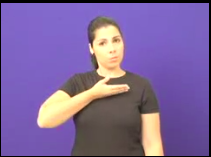
\includegraphics[height=3cm, width=5cm]{src/images/amigo.png}}}%
%     \qquad
%     \subfloat[Desculpa]{{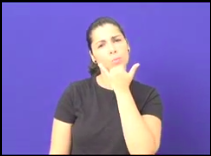
\includegraphics[height=3cm, width=5cm]{src/images/desculpa.png} }}%
%     \qquad
%     \subfloat[Telefone]{{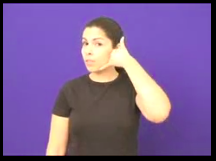
\includegraphics[height=3cm, width=5cm]{src/images/telefone.png} }}%
%     \qquad
%     \caption{Gestos selecionado para o conjunto de dados}%
%     \label{figure:gestos_selecionados}%
%     \fonte{Produção do autor} % Adaptado de Dicionário de Libras
% \end{figure}

% % Devo falar mais sobre a aplicação ?? (05/03/2019)
% \par A aquisição dos dados foi feita através de uma aplicação desenvolvida em Python (Figura \ref{figure:tela_inicial}) junto a biblioteca de criação de interfaces gráficas PyQt e a biblioteca de visão computacional OpenCV \cite{opencv2019}. Esta aplicação através da \textit{webcam} do usuário, adquire 60 imagens, sendo 20 de cada um dos gestos selecionados. Após a aquisição, as imagens são redimensionadas pela aplicação, para um formato 224x224x3 e então envia os arquivos das imagens por \textit{email}. O processo de redimensionamento é feito pois o algoritmo de treinamento da CNN recebe como entrada imagens no formato 224x224x3.

% % Ei!! Problema na imagem, você não declarou ter utilizado o gesto "Idade".... (07/03/2019)
% \image{0.60}{image_sistema_aquisicao_de_dados.png}{Tela inicial da aplicação de aquisição de dados}{figure:tela_inicial}{Produção do Autor}

% % Descrever que, foram onze colaboradores, porém foram utilizados dados de apenas 10 para o treinamento e 11 para o teste...
% % Assim deixo a coisa justa ao apresentar a matriz de confusão
% \par A aplicação foi distribuída para vários usuários e no total houveram onze colaboradores, com isto um total de 660 imagens foram coletadas, distribuídas igualmente entre todos os gestos.

% \subsection{Pré-processamento dos dados} 
% % Neste tópico acho que ainda está pouco claro o que foi feito... Rever depois, adicionando mais detalhes e imagens =D

% % Perguntar ao Sr. Claudio se a seleção de imagens boas e ruins entra no pré-processamento dos dados...
% % 07/03/2019 -> Falei com o Sr. Cláudio, e ele disse que está mesmo para pré-processamento...

% \par Após realizar a aquisição das imagens, cada uma delas foi avaliada para garantir que os gestos haviam sido feitos corretamente pelos colaboradores. Nesta etapa algumas imagens foram removidas do conjunto. A Figura (TTTY) apresenta a relação da quantidade de imagem com cada um dos gestos após a validação realizada.

% % ToDo: Criar o plot com a quantidade de imagens e os gestos....
% % Os dados: (Teste + Treino)
% %   - Amigo: 38 + 168
% %   - Desculpa: 19 + 160
% %   - Telefone: 38 + 151
% % Total: 574

% % ToDo: Criar parágrafo para falar sobre a divisão dos dados
% \par Com a validação do conjunto de dados realizada, o mesmo foi dividido em dados de treino e dados de teste, como forma de facilitar a validação da RNA, assim como citado anteriormente. Para este caso, um \textit{script} feito em Python (Figura \ref{figure:script_separacao_dados}), com o auxilio da biblioteca \textit{sklearn}, foi criado para separar os dados, de forma randômica, utilizando 80\% para o conjunto de treino e 20\% para o teste.

% % Preciso colocar o source do `move_data` ?
% \begin{figure}[H]
%     \centering
%     \begin{lstlisting}[language=Python]
% import os
% import numpy as np

% from shutil import copyfile

% from sklearn.model_selection import train_test_split

% x, y = [], []

% for root_dir in os.listdir():
%     files = os.listdir(root_dir)

%     x.extend(files)
%     y.extend(np.repeat(root_dir, len(files)))

% x_train, x_test, y_train, y_test = train_test_split(x, y, \ test_size=0.20, random_state=992)

% move_dados(x_train, y_train, 'treino')
% move_dados(x_test, y_test, 'teste')

%     \end{lstlisting}
%     \caption{\textit{Script} para separar os dados de treino e teste}
%     \label{figure:script_separacao_dados}
% \end{figure}

% % Colocar alguma referência no Data Augmentation...
% % Mudar isto, talvez falar apenas que é um conjunto pequeno....
% \par O conjunto de dados adquiridos para o trabalho não é considerado grande, já que podem haver muitas variações principalmente no cenário e vestuário dos usuários, desta forma ao realizar a divisão, o conjunto utilizado no treino fica ainda menor, podendo haver problemas relacionados a \textit{Overfitting}. Para resolver este problema, foi aplicado a técnica de \textit{Data Augmentation}, que de acordo com \citeonline{Amidi2018Tricks} pode ser utilizado quando há conjuntos pequenos de dados para o treinamento de CNNs. Nesta técnica, imagens artificiais são criadas a partir do conjunto de testes, isto feito através da aplicação de filtros e distorções na imagem \cite{Amidi2018Tricks}.

% % Colocar o porque estas transformações foram escolhidas, acho que não.....
% Neste trabalho foi utilizado um \textit{Pipeline} de \textit{Data Augmentation} probabilístico, onde para cada filtro ou distorção há uma probabilidade de ser aplicado na imagem, no total 1500 imagens das três classes foram geradas. O \textit{script} foi criado em Python, e é apresentado na Figura \ref{figure:dataaugmentation}.

% \begin{figure}[H]
%     \centering
%     \begin{lstlisting}[language=Python]
% import Augmentor

% p = Augmentor.Pipeline('gestos_editados/treino')

% p.flip_left_right(probability=0.6)

% p.rotate(probability=0.7, max_left_rotation=3, max_right_rotation=3)
% p.rotate(probability=0.4, max_left_rotation=7, max_right_rotation=7)

% p.random_distortion(probability=0.5, grid_height=3, grid_width=3, magnitude=2)
% p.random_distortion(probability=0.4, grid_height=4, grid_width=4, magnitude=3)

% p.skew_left_right(probability=0.3, magnitude=0.7)
% p.skew_corner(probability=0.4, magnitude=0.5)

% p.shear(probability=0.5, max_shear_left=4, max_shear_right=3)

% p.sample(1500)
%     \end{lstlisting}
%     \caption{\textit{Script} para separar os dados de treino e teste}
%     \label{figure:dataaugmentation}
% \end{figure}

% % Sobre os dados do data augmentation
% %   - Amigo: 502
% %   - Desculpa: 524
% %   - Telefone: 474
% % Total: 1500

% % ToDo: Colocar exemplos de imagens geradas no Augmentation...
% % ToDo: Colocar as quantidades de imagem após o Data Augmentation...

% \subsection{Treinamento da Rede Neural Artificial}

% % ToDo: Falar sobre o retreino do Mobilenet
% %% Posso utilizar como base a exposição feita pelo Felipe....
% % ToDo: Falar sobre a exportação do modelo para o formato web...

% \subsection{Distribuição do modelo}

% % ToDo: O foco deste trabalho é aplicar o Deep Learning nas tecnologias Web, para isto uma API foi criada para a distribuição dos modelos utilizados na biblioteca.....
% % ToDo: Falar do Flask.
% % Rotas...
% % Código básico da API

% \section{Recurso assistivo para deficiência motora}

% % Estou em dúvidas sobre o que colocar aqui...

% % Falar que utilizei o trabalho do WebGazer como base, porém toda a identificação é feita utilizando o PoseNet....
% % Terá de fazer comparações ao Webgazer.js ? ? ? Acho que não, são coisas diferentes....
% % Falar sobre o OJ Ramos ??? Acho que sim...... Falar que ele gerou um produto com isto.....

% \subsection{Calibração}

% % ToDo: Falar sobre a API de calibração...
